\chapter{Resultados obtenidos para los proplyds ``clásicos''}
Probamos nuestro modelo descrito en los capítulos anteriores en una muestra de
proplyds pertenecientes a la Nebulosa de Orión (ONC) que presentan un choque de
proa. En la figura  se muestran los proplyds que pertencen a nuestra muestra.

En todos los casos no fue posible medir el radio característico $R_{90}$ debido a
que el brillo de la cáscara decae con el ángulo polar $\theta$ y no es detectale
para ángulos del orden de $60^\circ$. Sin embargo, a continuación mostraremos la
metodología para obtener la inclinación más probable de cada choque, así como los
parámetros del modelo de cada uno de éstos que nos indican su forma intrínseca.

\begin{figure*}
    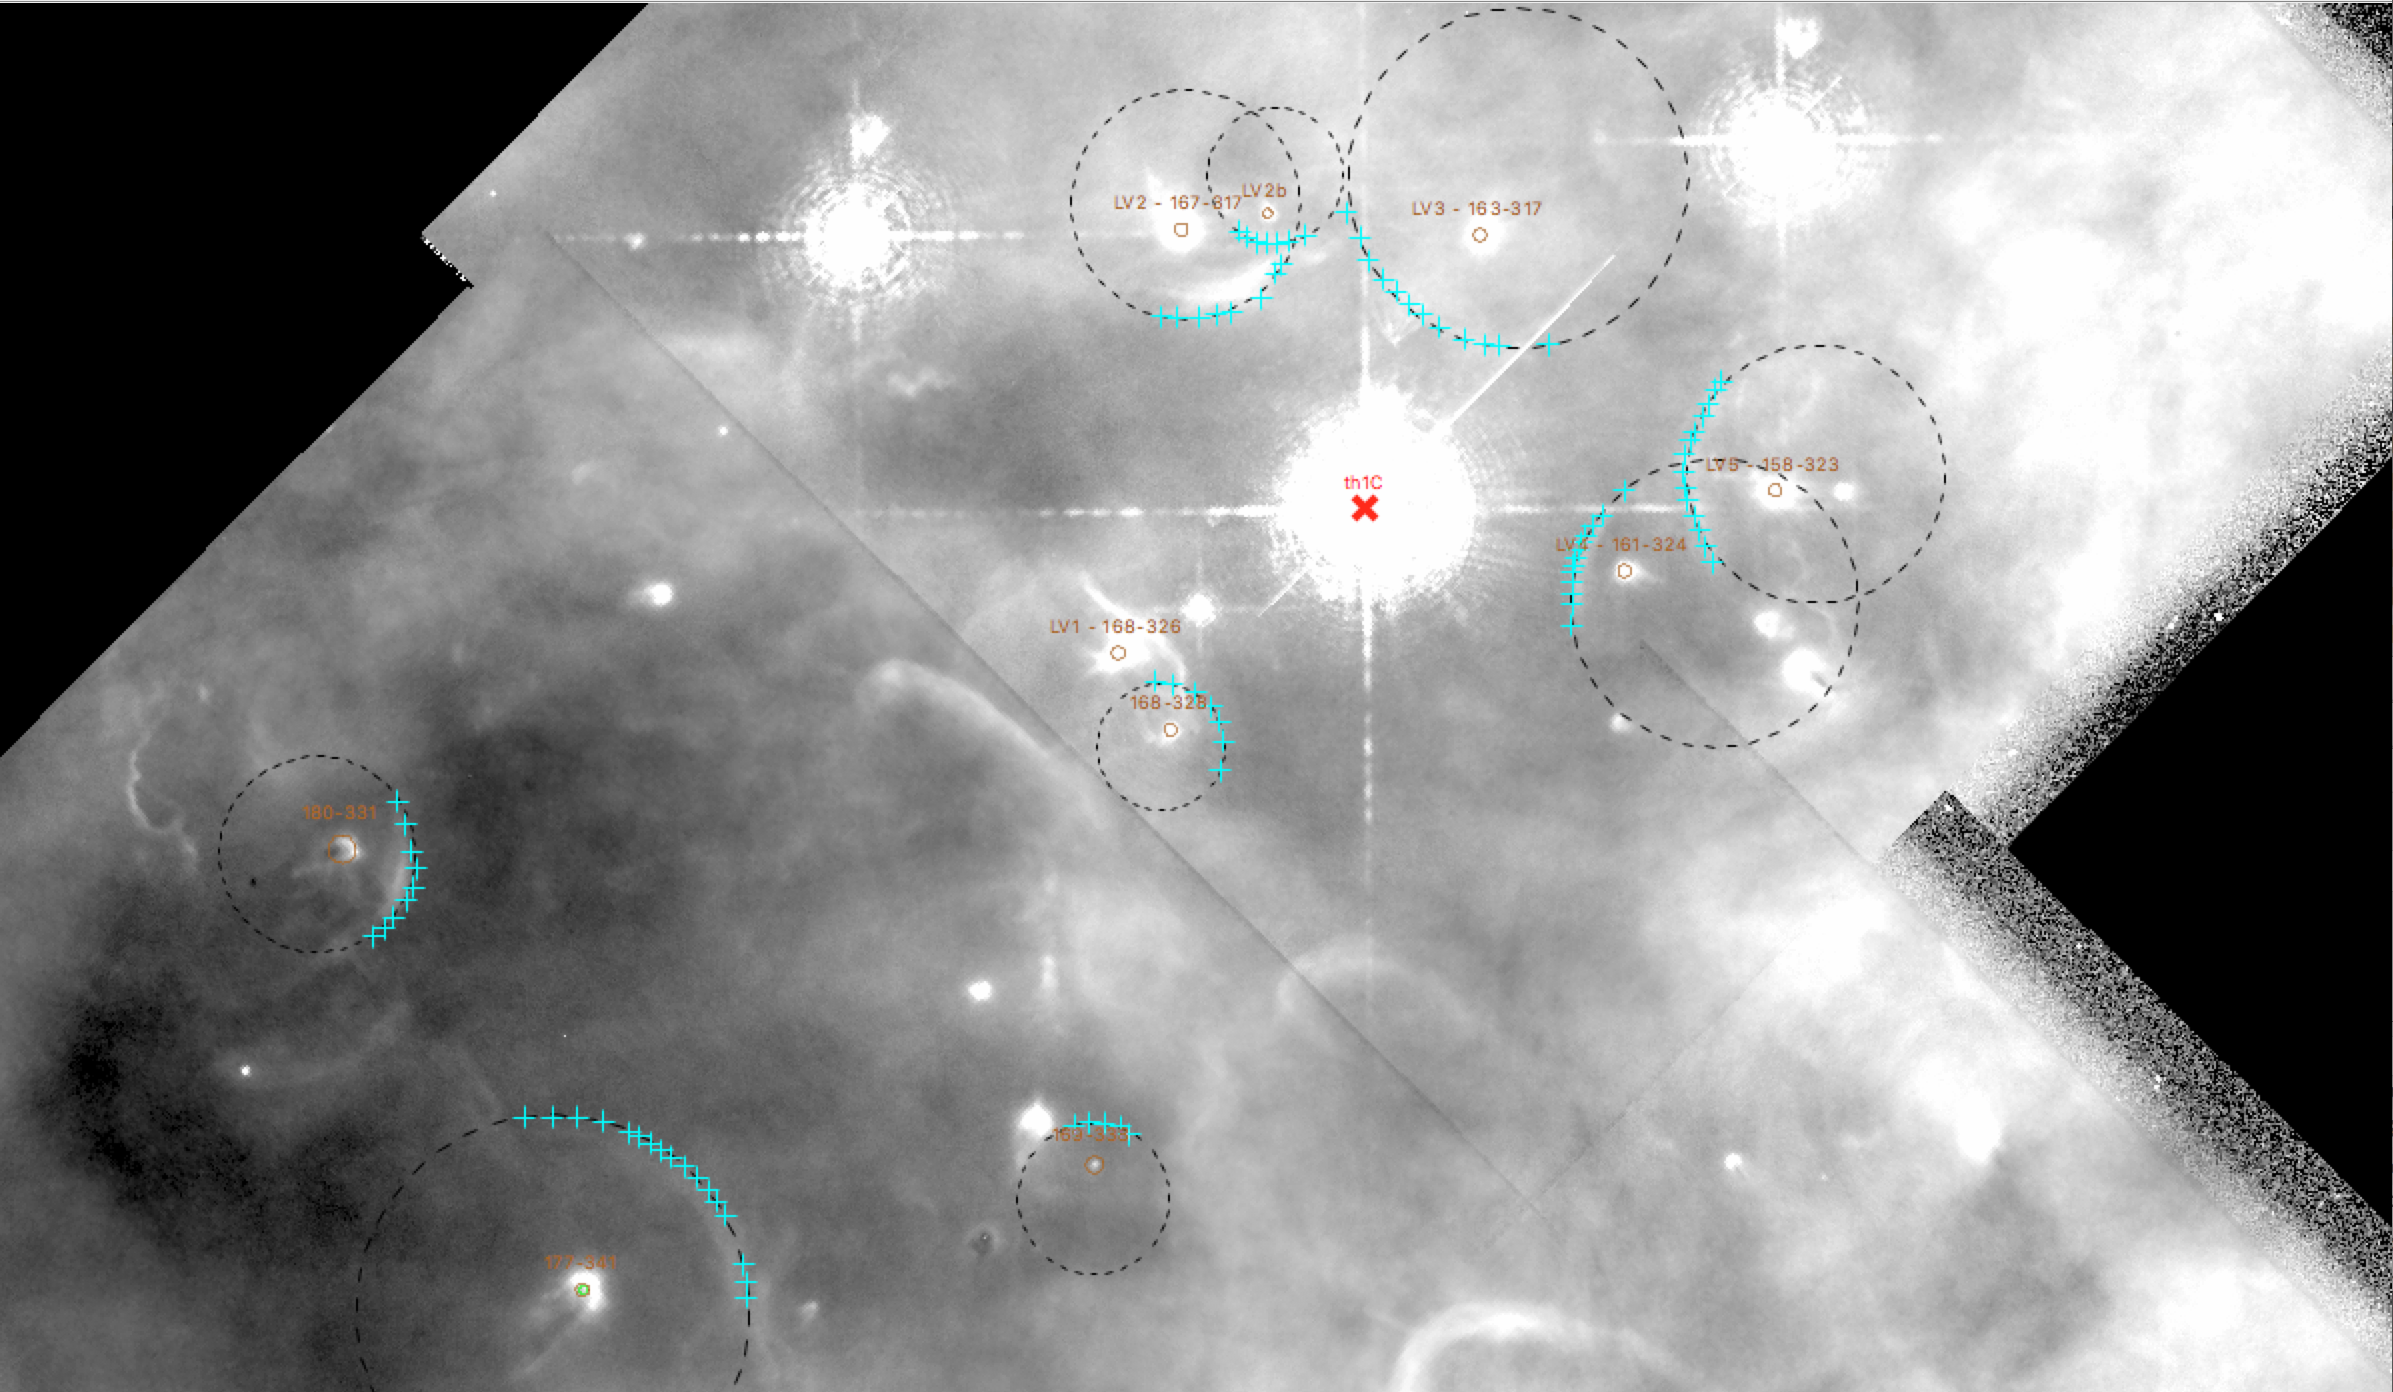
\includegraphics[width=\linewidth]{./Figures/LV-full-field-annotated}
    \caption{Imagen de la parte central de la Nebulosa de Orión donde se ubican
    los proplyds de nuestra muestra. Las cruces color cyan corresponden a las
    mediciones de la forma aparente para cada choque de proa. Los círculos
    amarillos marcan la posición de cada proplyd y la ``x'' roja corresponde a la posición de la estrella ionizante \thC{}. Los círculos negros ilustran de manera esquemática el radio de curvatura de cada choque.}
    \label{fig:proplyds-map}
\end{figure*}

\section{Metodología para la medición de la forma aparente.}
\label{sec:methodology}
Se utilizaron imágenes en el filtro de $[OIII]$ de la cámara WPC2 del Telescopio
Espacial Hubble (HST). Se utilizaron las herramientas del programa DS9 para
análisis de imágenes astronómicas para trazar la posición de \thC{} y de cada uno
de los proplyds de la muestra. La posición y la forma de los choques de proa fue
trazada con una serie de marcas a lo largo del choque. Las coordenadas de las marcas fueron guardadas en un archivo y luego procesadas para tener las
coordenadas del choque en el sistema de referencia del proplyd (Figura \ref{fig:proplyds-map}). El radio de curvatura aparente se obtiene haciendo un ajuste de mínimos cuadrados de la forma de un círculo de las mediciones obtenidas. $R_0$ se obtiene como la distancia mínima entre el proplyd y el ajuste circular dentro del rango de las coordenadas de las mediciones. 

\subsection{Medición de incertidumbres}

Para saber qué tan confiables son las coordenadas de las mediciones, se realizó
el procedimiento siguiente: Del total de mediciones realizadas para cada proplyd,
se crearon varias sub-muestras donde se utilizamos aproximadamente las dos terceras partes de las mediciones, pero dejando un mínimo de cuatro puntos, y se procedió a calcular los radios característicos para cada submuestra, y comprobar qué tanto se desvían estas mediciones de la original. En la figura \ref{fig:char-radii-obs} se muestran ejemplos de dichas sub-muestras para algunos proplyds.


\begin{figure*}
  \setkeys{Gin}{width=0.33\linewidth}%, trim=10 30 55 62.5}
\begin{tabular}{@{}c@{}c@{}c@{}}
 
Todos los puntos & Primera sub-muestra & Segunda sub-muestra \\ 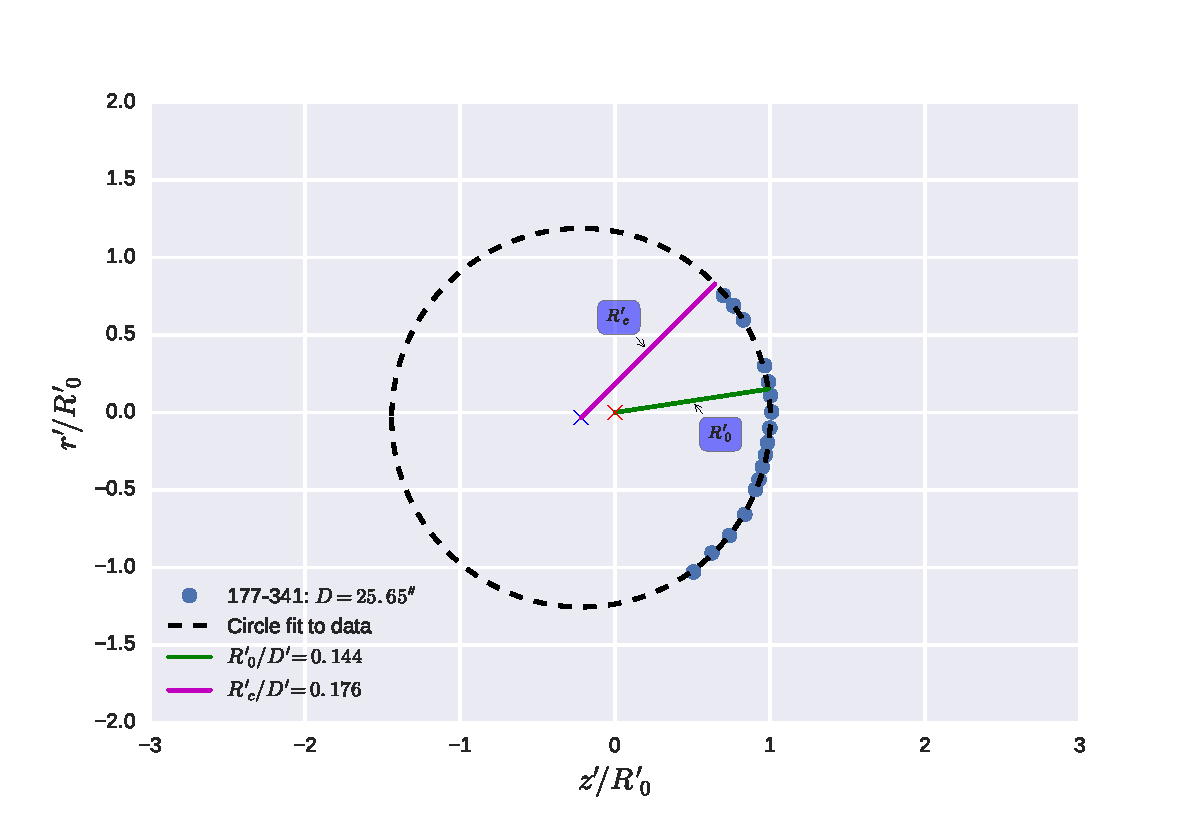
\includegraphics[clip]{./Figures/LV-bowshocks-xyfancy-positionswill-177-341} & 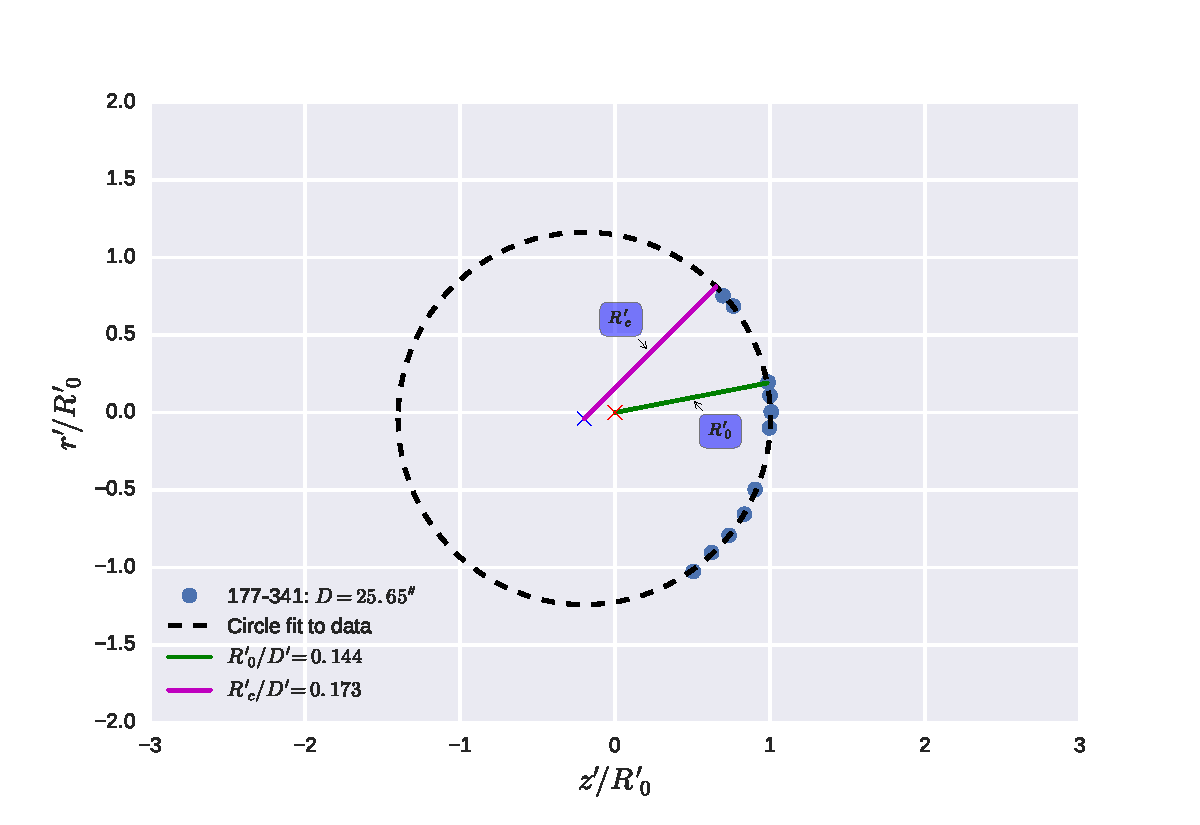
\includegraphics[clip]{./Figures/LV-bowshocks-xyfancy-positionssamp00-177-341} &
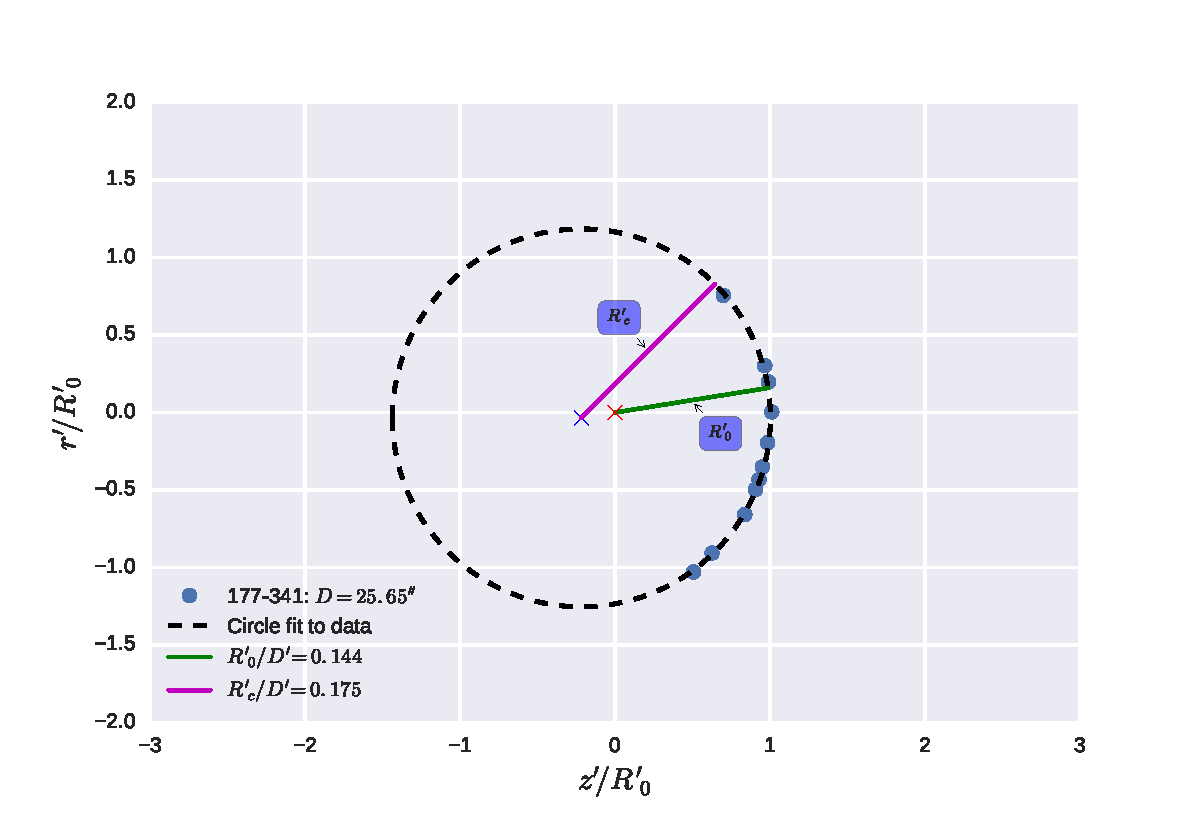
\includegraphics[clip]{./Figures/LV-bowshocks-xyfancy-positionssamp01-177-341} \\
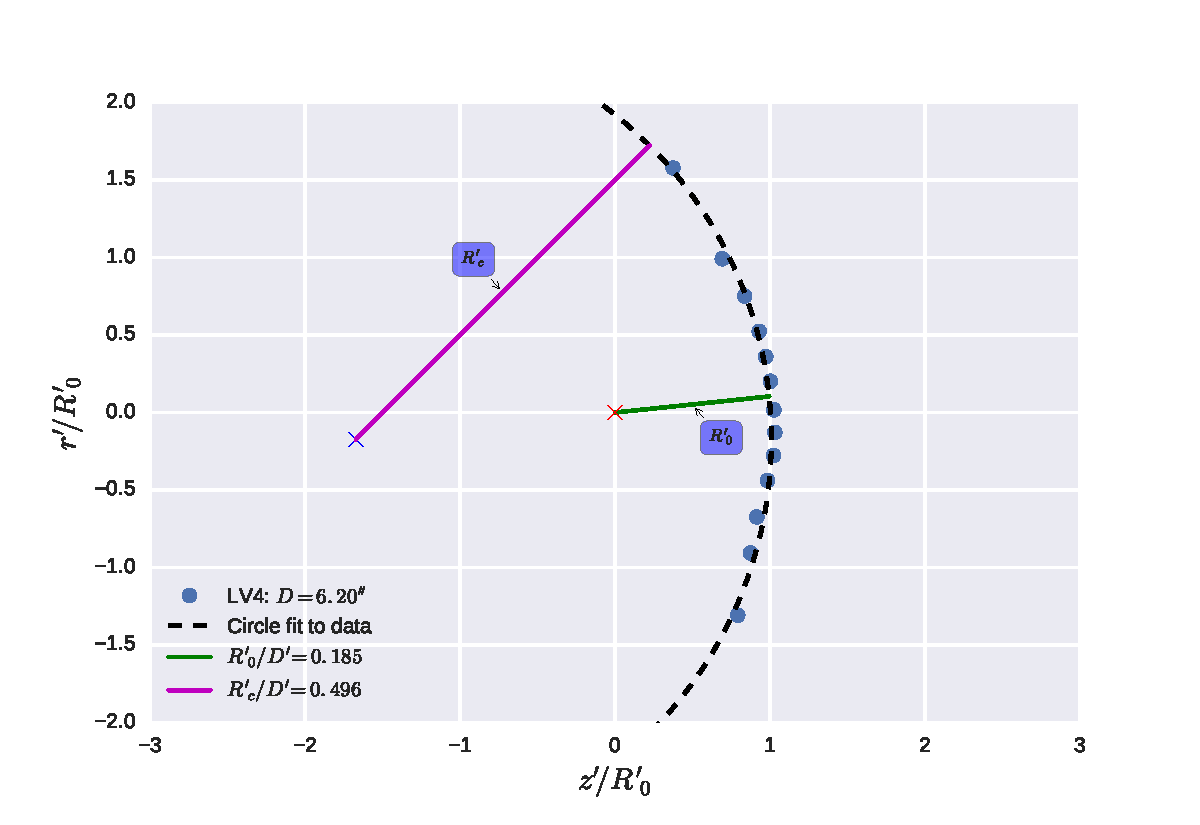
\includegraphics[clip]{./Figures/LV-bowshocks-xyfancy-positionswill-LV4} & 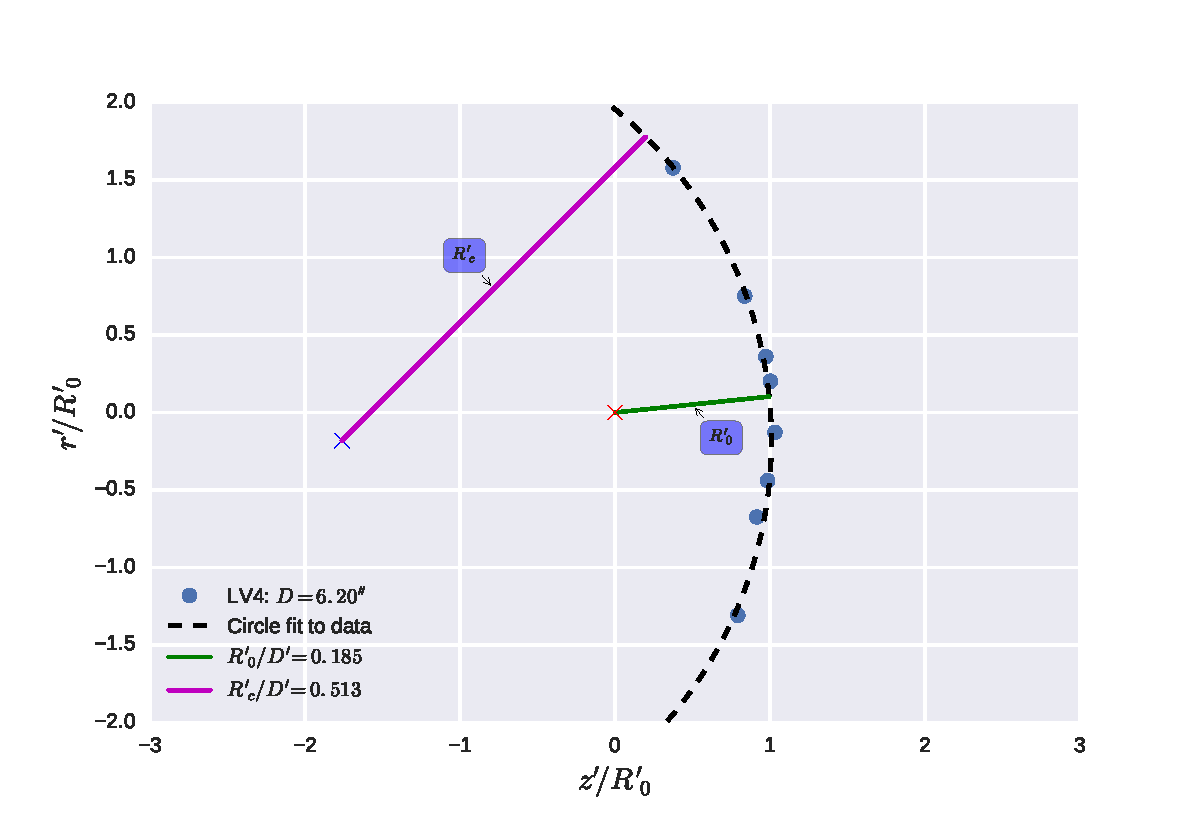
\includegraphics[clip]{./Figures/LV-bowshocks-xyfancy-positionssamp00-LV4} & 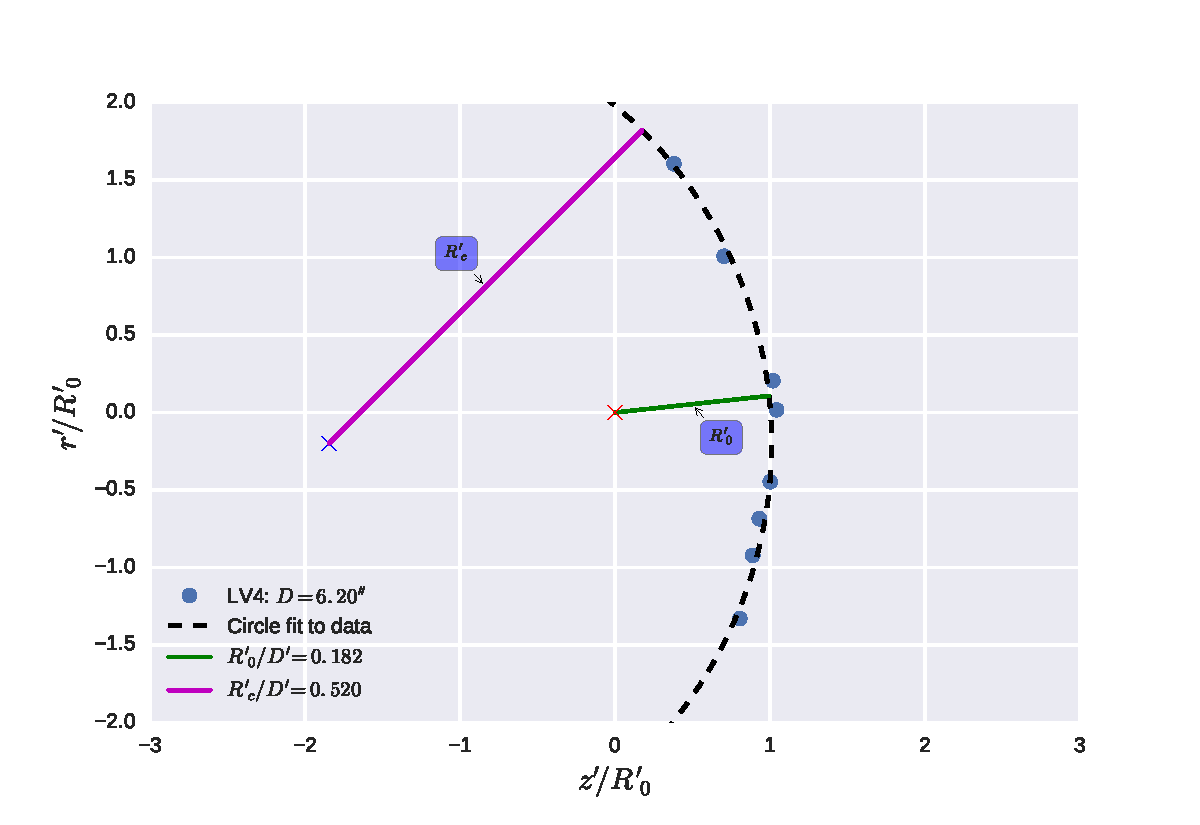
\includegraphics[clip]{./Figures/LV-bowshocks-xyfancy-positionssamp01-LV4} \\
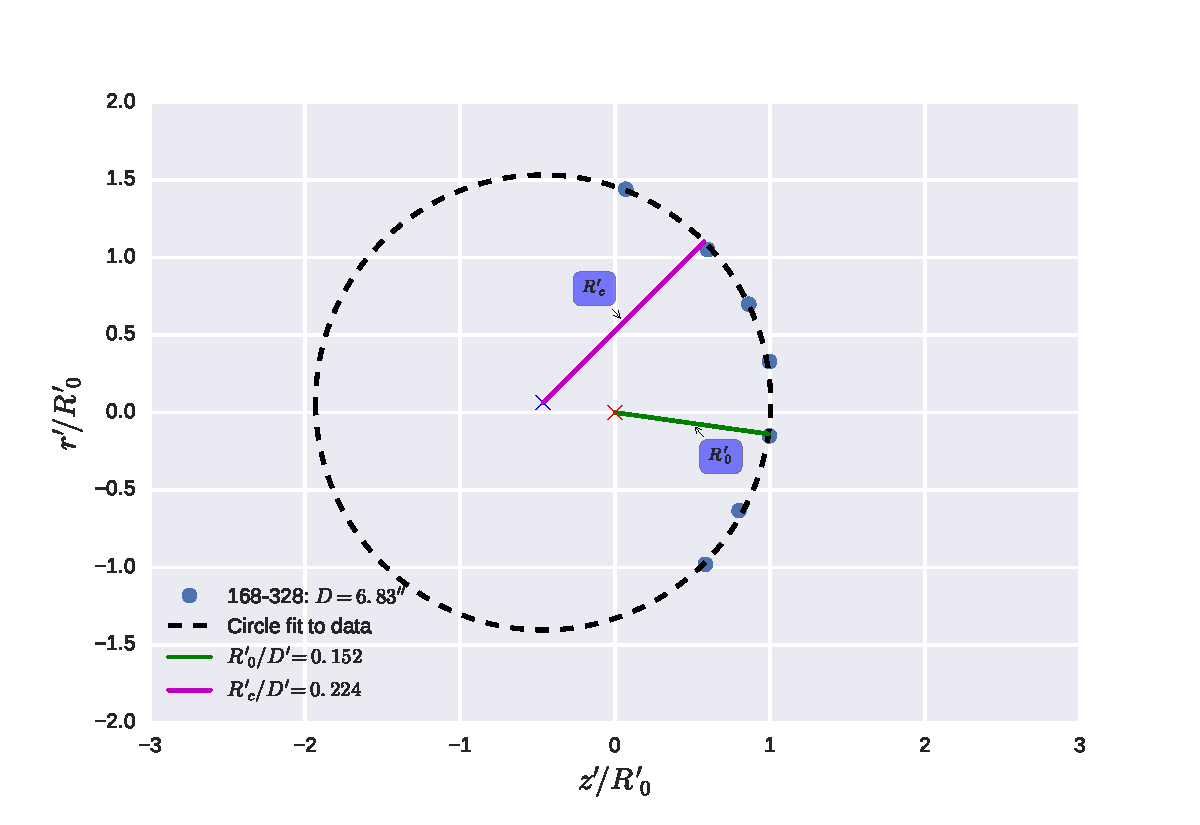
\includegraphics[clip]{./Figures/LV-bowshocks-xyfancy-positionswill-168-328} &  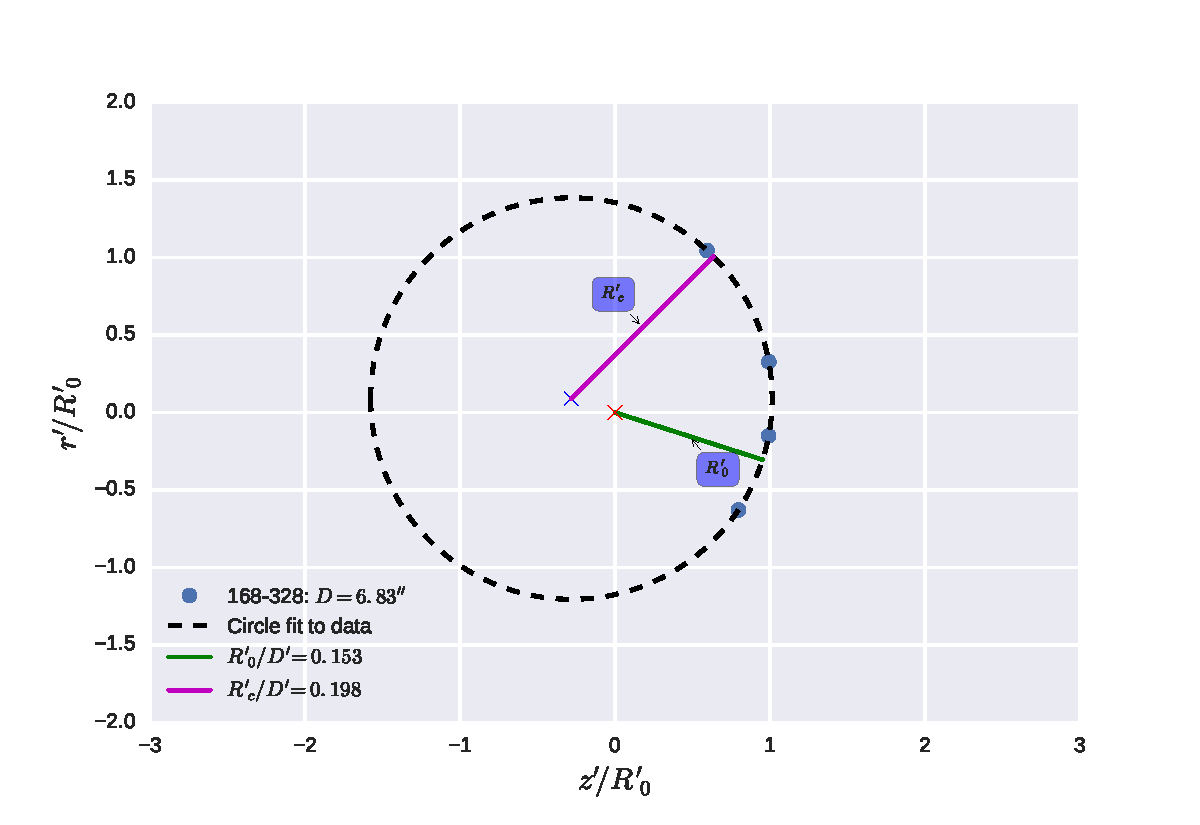
\includegraphics[clip]{./Figures/LV-bowshocks-xyfancy-positionssamp00-168-328} & 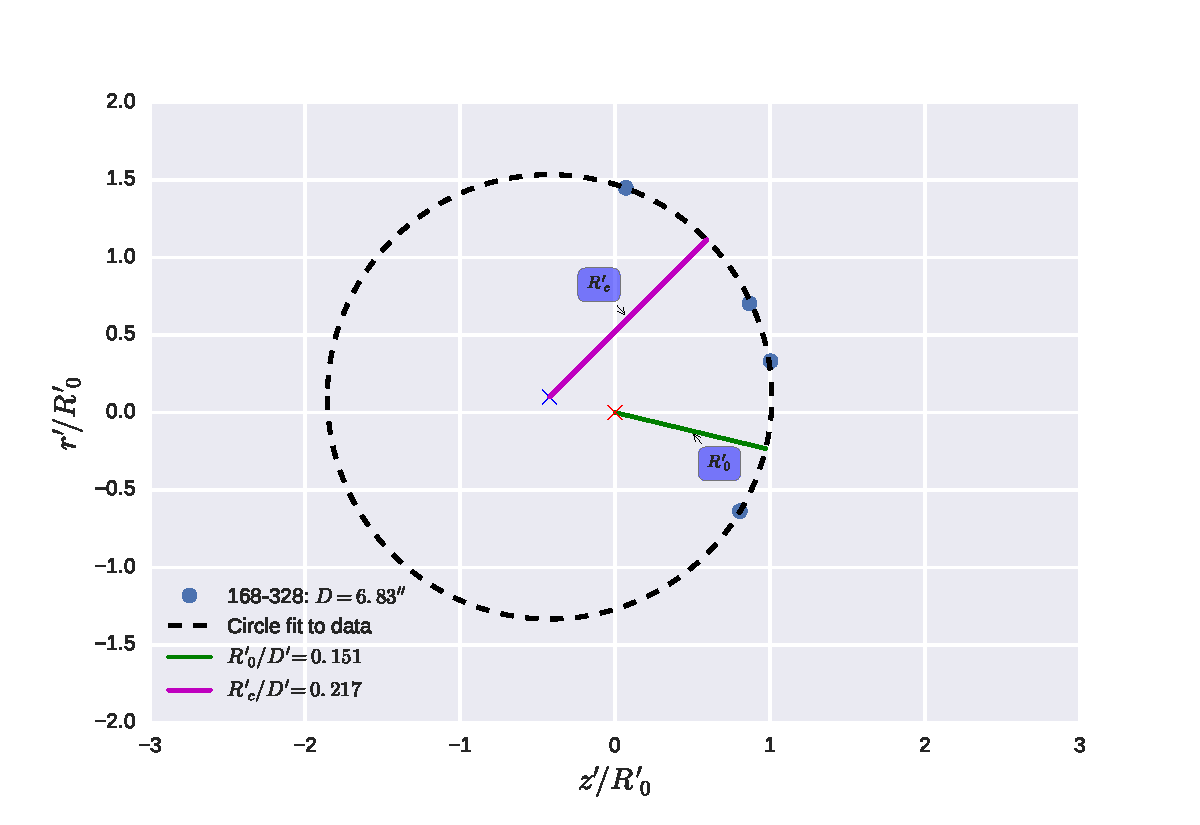
\includegraphics[clip]{./Figures/LV-bowshocks-xyfancy-positionssamp01-168-328}
\end{tabular}
\caption{Ejemplos de incertidumbres sistemáticas en los ajustes circulares a la forma de los choques para tres fuentes (desde la línea superior hasta la inferior): 177-341, LV4 y 168-328. La columna de la izquierda muestra el ajuste a todos los puntos identificados en el borde de la cáscara, donde el número y el espaciamiento de los puntos es una medida subjetiva de nuestra confianza al trazar el borde de cada cáscara. Las dos columnas restantes muestran ajustes a sub-muestras seleccionadas aleatoriamente que contienen 2/3 partes de los puntos de la muestra original para cada cáscara.}
\label{fig:char-radii-obs}
\end{figure*}

\section{Resultados}

Los radios característicos obtenidos para la muestra original y para las submuestras se muestran en la figura \ref{fig:conic-xi}. En cada pánel se utiliza un valor fijo para el parámetro de anisotropía $\xi$. Las mediciones para el proplyd LV4 son consistentes con un viento isotrópico, mientras que para los proplyds LV2b, 169-338, 180-331, 168-328, 177-341, LV3 y LV5 sus mediciones son consistentes para vientos con un grado de anisotropía bajo $(\xi \gtrsim 0.8)$. Finalmente para LV2 sus mediciones son consistentes con un viento con un grado de anisotropía alto $(\xi \lesssim 0.4)$. 

\begin{figure*}
\begin{tabular}{cc}
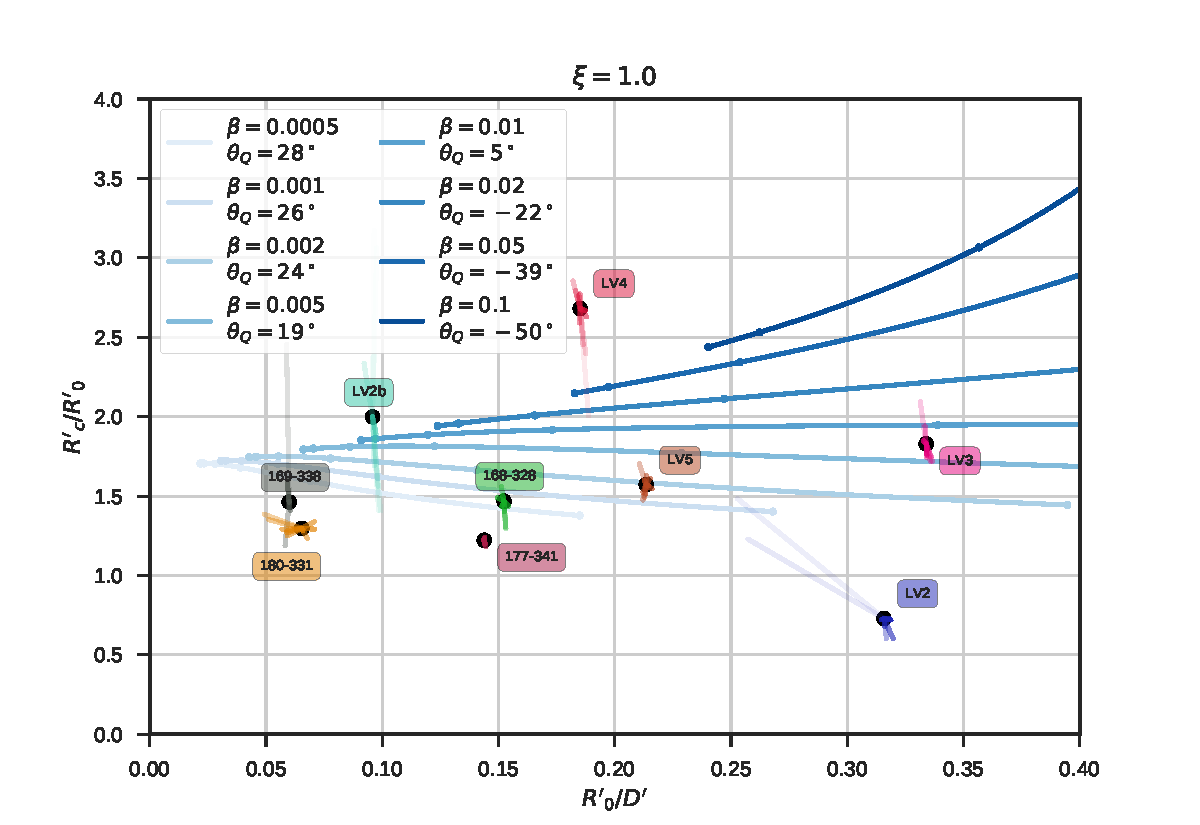
\includegraphics[width=0.48\linewidth]{./Figures/conic_xi-10} & 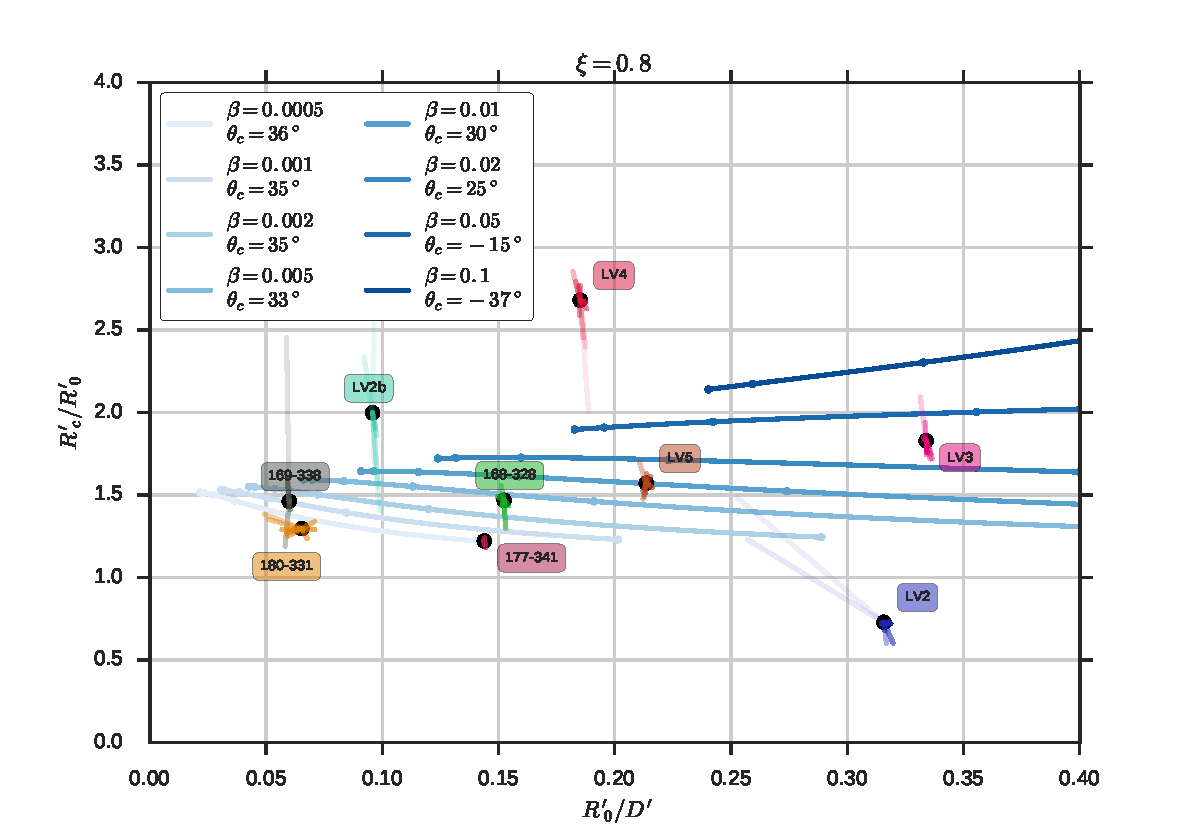
\includegraphics[width=0.48\linewidth]{./Figures/conic_xi-08} \\
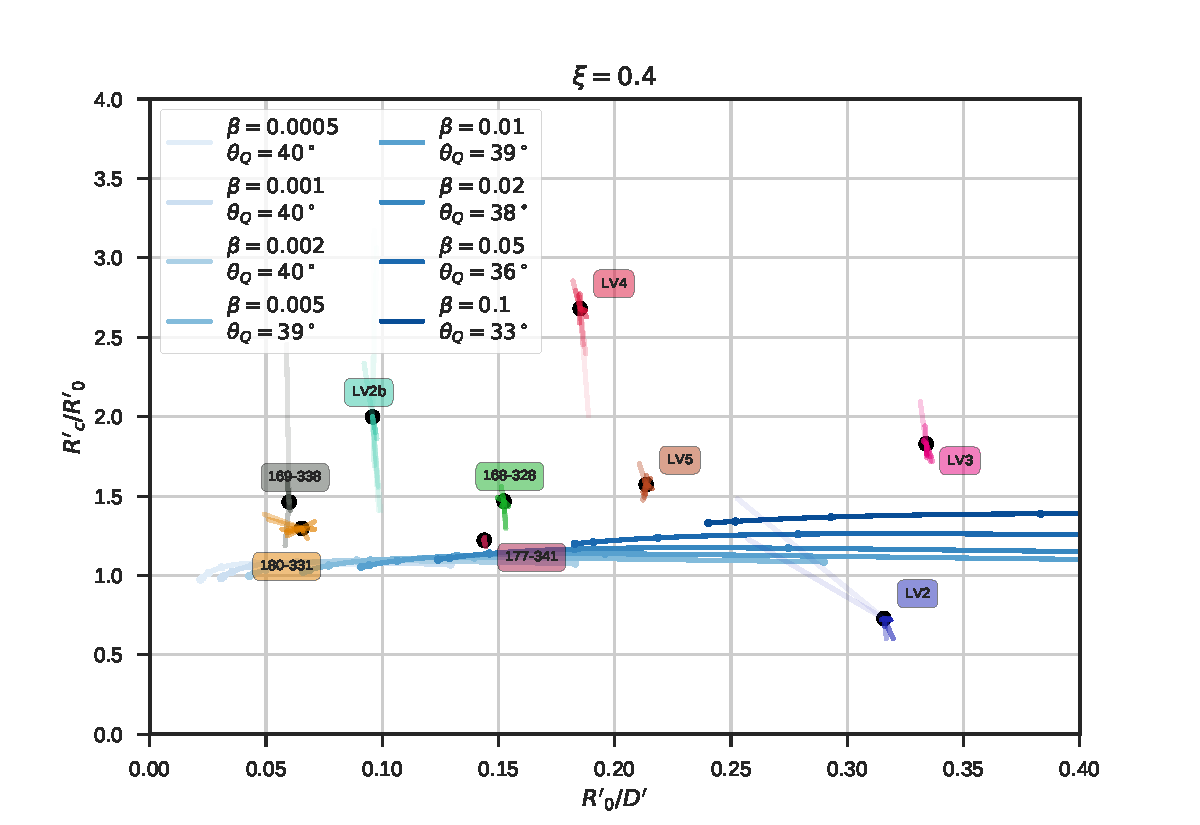
\includegraphics[width=0.48\linewidth]{./Figures/conic_xi-04} & 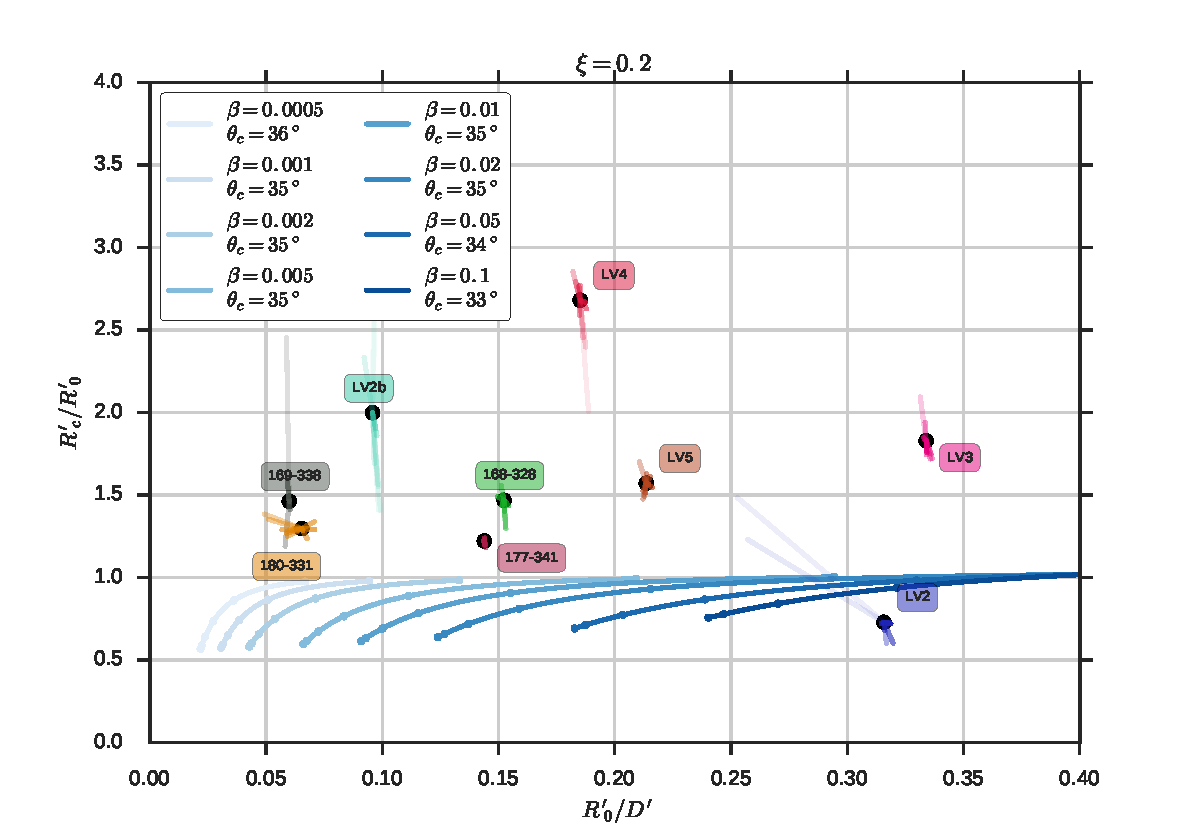
\includegraphics[width=0.48\linewidth]{./Figures/conic_xi-02} 
\end{tabular}
\caption{Mediciones de los radios característicos de los proplyds $R_c$ y $R_0$. Las curvas representan el ajuste de una cuádrica para un choque de proa con un cociente de momentos $\beta$ fijo, además se muestra su respectivo valor de $\theta_c$. Los puntos a lo largo de cada curva representan una separación en inclinación de $15^\circ$. Las mediciones para cada proplyd vienen acompañadas con el set de sub-muestras representadas como líneas radiales de colores. En cada gráfica se utiliza un valor diferente para el parámetro de anisotropía $\xi$, iniciando con un viento isotrópico $(\xi=1)$, hasta el viento  con mayor anisotropía $(\xi=0.2)$.}
\label{fig:conic-xi}
\end{figure*}

Con base a este análisis, se resume en la tabla \ref{tab:arc-fits} los ajustes a los parámteros de los proplyds: inclinación, distancia a \thC{} intrínseca $D$ y radio del choque en el eje de simetría $R_0/D$.

\begin{table*}
  \caption{Ajuste a los parámetros de los arcos para los choques de proa de los proplyds}
  \label{tab:arc-fits} 
\newcommand\C[1]{\multicolumn{1}{c}{#1}}
\begin{tabular}{llrllllrlll}\toprule
             &          & \multicolumn{3}{c}{\dotfill Obsetvado \dotfill}              & \multicolumn{6}{c}{\dotfill Ajuste teórico \dotfill} \\ 
  \C{OW}     & \C{Nombre} & \(D'\) &\C{ \(R_0'/D'\) }&\C{ \((R_c'/R_0')_{\mathrm{shape}}\) }&\C{ \((R_c'/R_0')_{\mathrm{flux}}\) }&\C{ \(\beta\) }&\C{ \(\xi\) }&\C{ \(|i|\) }&\C{ \(D\) }&\C{ \(R_0/D\)}\\
  \C{(1)}& \C{ (2) }&\C{ (3)    }&\C{    (4)      }&\C{              (5)           }&\C{           (6)             }&\C{     (7)   }&\C{   (8)   }&\C{   (9) }&\C{  (10) }&\C{   (11)} \\
\midrule     
 168-328  &            &    6.8  &  $0.152 \pm 0.001$  &  $1.42 \pm 0.09$   &  $1.45 \pm 0.05$     &  $0.018 \pm 0.003$  &  0.4 -- 0.6  &  $33 \pm 3$   &  $0.017 \pm 0.001$  &  $0.115 \pm 0.005$  \\
 169-338  &            &  16.4  &  $0.059 \pm 0.001$  &  $1.76 \pm 0.48$   &  $1.50 \pm 0.05$     &  $0.002 \pm 0.001$  &  0.8 -- 0.8  &  $43 \pm 8$   &  $0.049 \pm 0.006$  &  $0.035 \pm 0.005$  \\
 177-341  & HST1   & 25.6  &  $0.144 \pm 0.001$  &  $1.21 \pm 0.02$   &  $1.25 \pm 0.02$     &  $0.018 \pm 0.003$  &  0.1 -- 0.2  &  $30 \pm 5$   &  $0.064 \pm 0.003$  &  $0.115 \pm 0.005$  \\
 180-331  &             &  25.1  &  $0.061 \pm 0.007$  &  $1.30 \pm 0.05$   &  $1.27 \pm 0.05$     &  $0.003 \pm 0.001$  &  0.4 -- 0.4  &  $35 \pm 7$   &  $0.066 \pm 0.007$  &  $0.047 \pm 0.005$  \\
 167-317  &  LV2     &    7.8  &  $0.305 \pm 0.025$  &  $0.81 \pm 0.28$   &  $1.50 \pm 0.1$      &  $0.085 \pm 0.015$  &  0.1 -- 0.2  &  $13 \pm 13$  &  $0.017 \pm 0.001$  &  $0.225 \pm 0.005$  \\
               & LV2b    &   7.2  &  $0.097 \pm 0.002$  &  $2.00 \pm 0.62$   &  $1.63 \pm 0.08$     &  $0.008 \pm 0.003$  &  0.8 -- 0.8  &  $28 \pm 13$  &  $0.018 \pm 0.002$  &  $0.078 \pm 0.013$  \\
 163-317  & LV3      &   6.9  &  $0.334 \pm 0.002$  &  $1.81 \pm 0.12$   &  $1.85 \pm 0.15$     &  $0.075 \pm 0.025$  &  0.6 -- 0.8  &  $35 \pm 5$   &  $0.018 \pm 0.001$  &  $0.205 \pm 0.025$  \\
 161-324  & LV4      &   6.2  &  $0.186 \pm 0.002$  &  $2.59 \pm 0.24$   &  $2.05 \pm 0.07$     &  $0.040 \pm 0.014$  &  0.8 -- 1.0  &  $18 \pm 12$  &  $0.014 \pm 0.001$  &  $0.160 \pm 0.028$  \\
 168-323  & LV5      &   9.6  &  $0.213 \pm 0.002$  &  $1.57 \pm 0.07$   &  $1.60 \pm 0.07$     &  $0.055 \pm 0.005$  &  0.2 -- 0.4  &  $20 \pm 5$   &  $0.022 \pm 0.001$  &  $0.190 \pm 0.010$  \\
\bottomrule
\end{tabular}
\begin{minipage}{0.95\linewidth}
  Notes --
%
  Col.~(1): ID de la fuente \citep{ODell:1994a}.
%
  Col.~(2): Nombre alternativo de la fuente.
% 
  Col.~(3): Distancia proyectada desde \thC{}, segundos de arco.
%
  Col.~(4): Radio exterior aparente a lo largo del eje, normalizado con la distancia proyectada, con una incertidumbre de \(\pm 1\sigma\), determinado con el ajuste circular decrito en \S~\ref{sec:methodology}.
% 
  Col.~(5): Radio de curvatura aparente, normalizado con el radio a lo largo del eje, con incertidumbres de \(\pm 1\sigma\), determinado con el ajuste circular descrito en \S~\ref{sec:methodology}.
% 
  Col.~(6): Igual que Col.~(5) pero aplicando el criterio adicional de que el brillo superficial del proplyd obtenido debe coincidir con la predicción teórica.
%
  Col.~(7): Cociente de momentos entre el viento del proplyd y la estrella O (ver capítulo \ref{chap:hipersonica}). 
% 
  Col.~(8): Parámetro de anisotropía del viento del proplyd.
% 
  Col.~(9): Inclinación respecto al plano del cielo, en grados.
% 
  Col.~(10): Distancia real desde \thC{}, parsecs.
%
  Col.~(11): Radio real de la cáscara a lo largo del eje, normalizado con distancia.

\end{minipage}
\end{table*}
